\subsection{Gaussian Mixture Model}
We consider approximating a 10-D Gaussian mixture model with single mode and muti-modes(two components, weighted by 1/3 and 2/3 respectively.)
To investigate the faster convergence of accelerated variants of algorithms in the DPVI framework, 
we evaluated their performance to their non-accelerated counterparts in different hyperparameter settings
, by using the 2-Wasserstein ($W_2$) distance between the empirical distribution 
generated by each algorithm and the target distribution as a measure of convergence.
We generate 5,000 samples from the target distribution $\pi$ as reference to evaluate the $W_2$ distance by using the POT library.

In Figures \ref{fig1:entire_figure}, we plot the $W_2$ w.r.t iteration of fix weight Blob algorithms,
 continuous adjust weight Blob algorithms and duplicate/kill Blob algorithms. 
It can be observed that acceleration technics contribute to faster convergence in both Blob/Blob-CA/Blob-DK algorithms 
under different step size, fixing acceleration hyperparameter $\gamma$ to be 0.7 or 0.8.

\begin{figure}
    \centering
    \begin{subfigure}[b]{0.35\textwidth}
        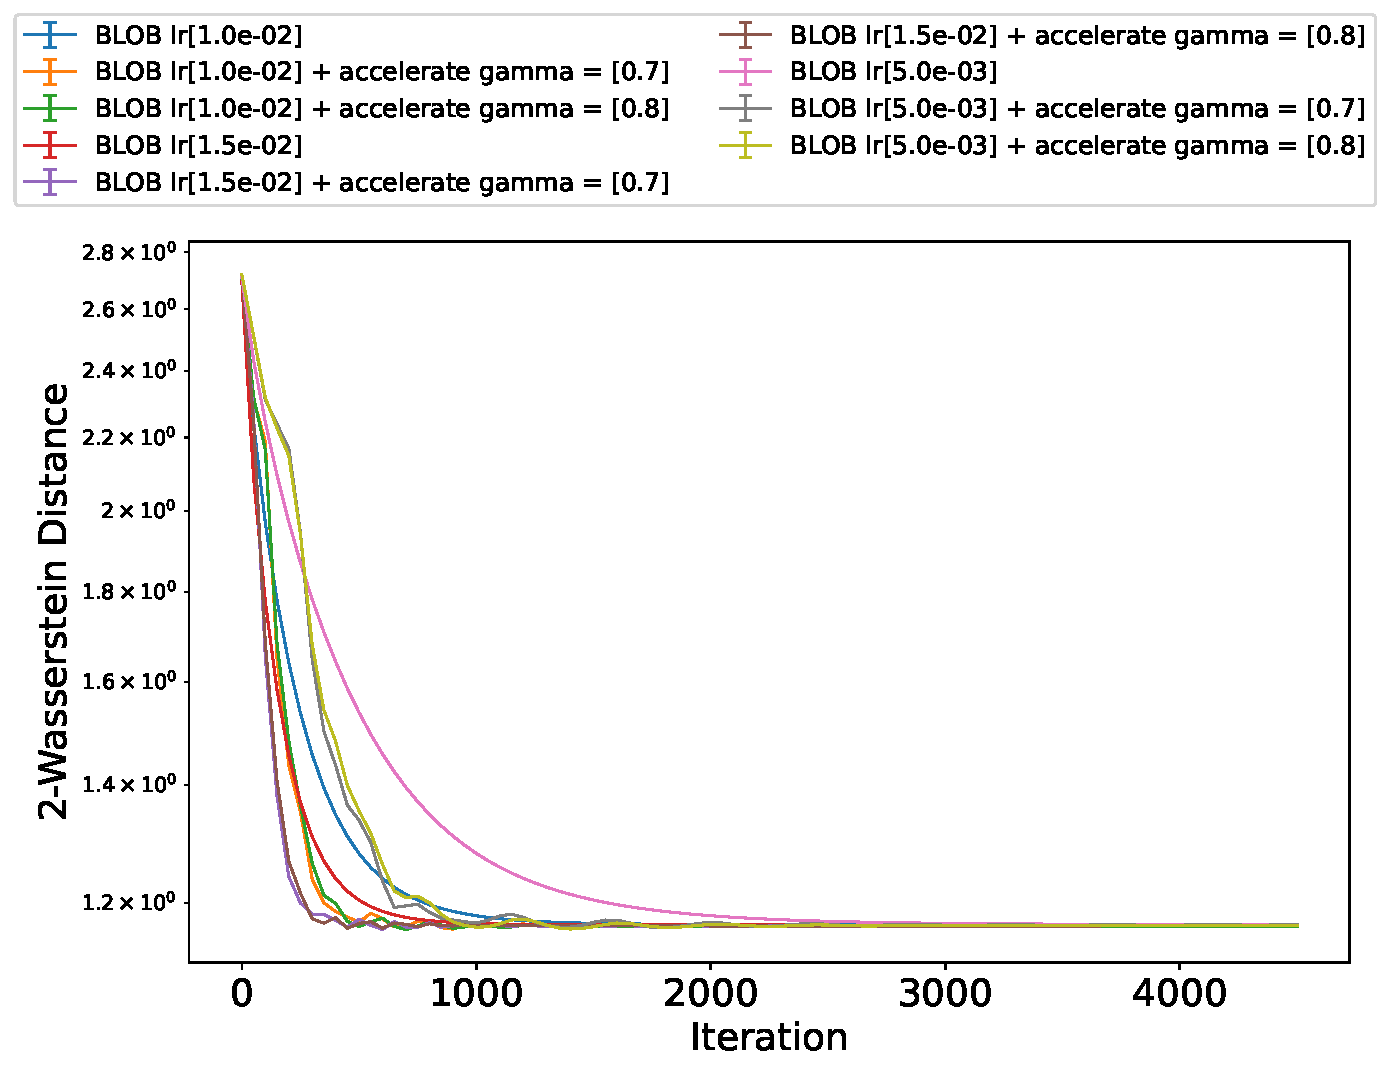
\includegraphics[width=\textwidth]{experiment_figure/GMM/demo_w2_Blob_acce_sg.pdf}
        \caption{fix weight}
        \label{fig1:image1}
    \end{subfigure}
    \hfill
    \begin{subfigure}[b]{0.35\textwidth}
        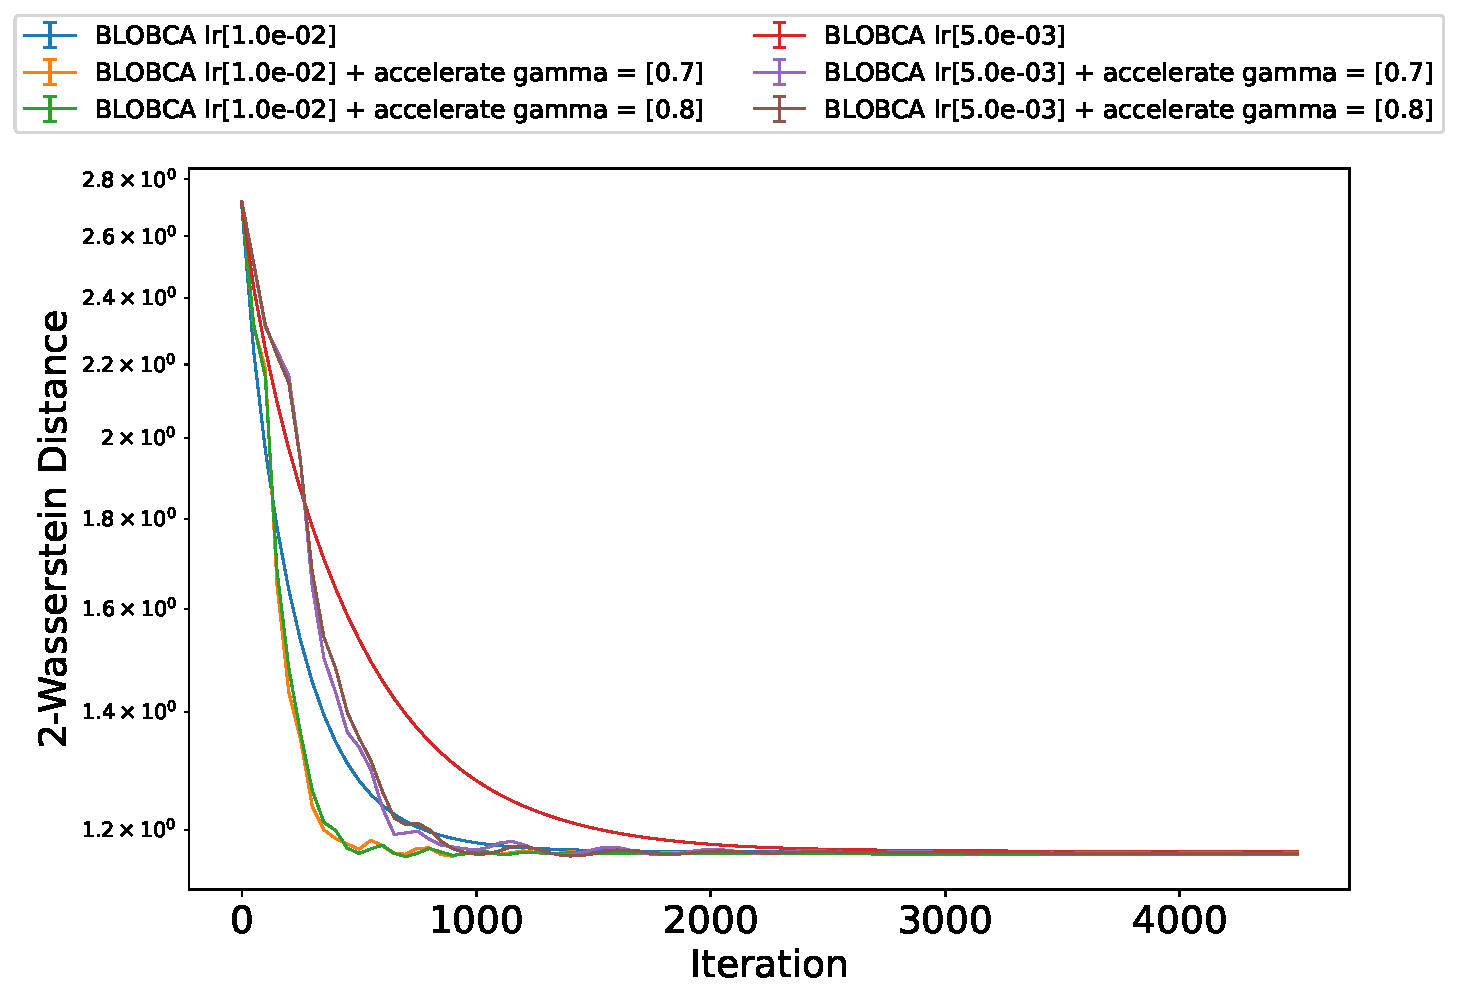
\includegraphics[width=\textwidth]{experiment_figure/GMM/demo_w2_BlobCA_acce_sg.pdf}
        \caption{continuous adjust weight}
        \label{fig1:image2}
    \end{subfigure}
    \hfill
    \begin{subfigure}[b]{0.35\textwidth}
        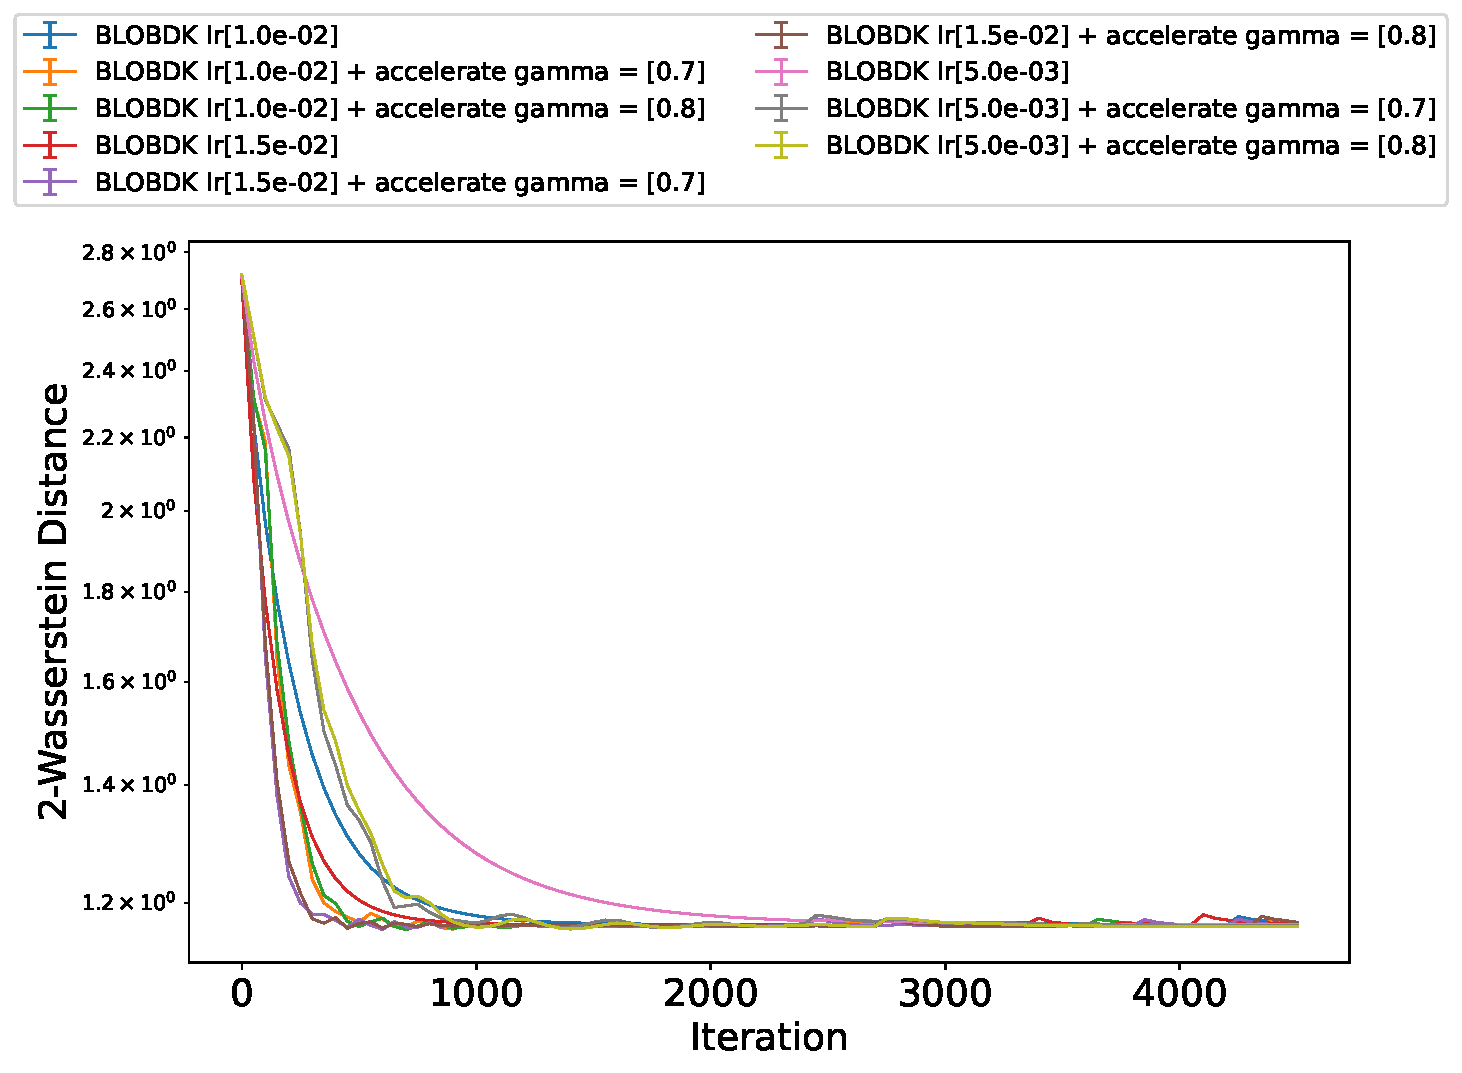
\includegraphics[width=\textwidth]{experiment_figure/GMM/demo_w2_BlobDK_acce_sg.pdf}
        \caption{duplicate/kill }
        \label{fig:image3}
    \end{subfigure}
    \caption{$W_2$ distance to the target w.r.t. iterations}
    \label{fig1:entire_figure}
\end{figure}








